% ============================================================================
\section{Acoustic features and training}
% ============================================================================

% --- Stanford CS224S lec9, slide 17 ---
\begin{frame}{Hidden Markov Model (HMM) basics}
  \begin{columns}[T,onlytextwidth]
    \begin{column}{0.52\textwidth}
      \begin{itemize}
        \item \textbf{Markov assumption:}
        \[
          P(q_t \mid q_1, \ldots, q_{t-1}) = P(q_t \mid q_{t-1})
        \]
        \item \textbf{Output-independence assumption:}
        \[
          P(o_t \mid O_1^{t-1}, q_1^t) = P(o_t \mid q_t)
        \]
      \end{itemize}
    \end{column}
    \begin{column}{0.48\textwidth}
      \begin{beamercolorbox}[rounded=true, leftskip=0.7em, rightskip=0.7em, sep=0.7em, colback=gray!10]{}
      {\scriptsize
      \begin{description}
        \item[$Q = q_1, \ldots, q_T$] a set of $N$ states
        \item[\textit{A} $= a_{ij}$:] \textbf{transition probability matrix} $A$, each $a_{ij}$ representing the probability of moving from state $i$ to state $j$. $\sum_j a_{ij} = 1\ \forall i$
        \item[$O = o_1, \ldots, o_T$] a sequence of $T$ observations, each one drawn from a vocabulary $V = v_1, \ldots, v_W$
        \item[$B = b_j(o_t)$] a sequence of \textbf{observation likelihoods}, also called \textit{emission probabilities}, each expressing the probability of an observation $o_t$ being generated from a state $j$
        \item[$q_0$, $q_F$] a special \textbf{start state} and (\textbf{final}) \textbf{end state} that are not associated with observations, together with transition probabilities $a_{q_0i}$ out of the start state and $a_{j q_F}$ into the end state
      \end{description}
      }
      \end{beamercolorbox}
 
    \end{column}
  \end{columns}
\end{frame}

% --- Stanford CS224S lec9, slide 15 ---
\begin{frame}{Hidden Markov Model (HMM) basics}
  \begin{itemize}
    \item \textbf{Objective function for DNN training: per-frame classification}
    \item Supervised learning: minimize classification errors at each time frame.
    \item \textbf{Standard choice: Cross entropy loss function}
      \begin{itemize}
        \item Extension of logistic loss for multiclass problems.
        \item For $K$ classes, target label $y$, input $x$, model parameters $W, b$:
        \[
          \mathrm{Loss}(x, y; W, b) = - \sum_{k=1}^K \mathbb{I}(y = k) \log f(x)_k
        \]
        $f(x)_k$: predicted probability for class $k$ at input $x$
      \end{itemize}
    \item This is a \textbf{frame-wise} loss: uses a label for each acoustic frame (from forced alignment).
    \item Other loss functions are possible, including ones that incorporate full-sequence or word error rate criteria, or deeper integration with HMMs.
  \end{itemize}
\end{frame}

\begin{frame}{HMM-GMM Decoding Architecture: Main Components}
  \begin{itemize}
    \item \textbf{Feature Extraction:}
      \begin{itemize}
        \item 39 MFCC features
      \end{itemize}
    \item \textbf{Acoustic Model:}
      \begin{itemize}
        \item Gaussian mixture models (GMM) to approximate $p(o|q)$
      \end{itemize}
    \item \textbf{Lexicon/Pronunciation Model:}
      \begin{itemize}
        \item HMM: which phones can follow each other. Sequence constraints from phonetic lexicon
      \end{itemize}
    \item \textbf{Language Model:}
      \begin{itemize}
        \item N-grams for computing $p(w_i|w_{i-1})$
      \end{itemize}
    \item \textbf{Decoder:}
      \begin{itemize}
        \item Viterbi algorithm: dynamic programming for combining all pieces to estimate a word sequence from audio
      \end{itemize}
  \end{itemize}
  \vfill
  \slideimgsource{Stanford CS224S, Lecture 9 (2025 Spring), slide 15 (adapted).}
\end{frame}

% --- Stanford CS224S lec9, slide 18 ---
\begin{frame}{Simple HMM: Estimating climate from ice cream observations}
  \textbf{You are a climatologist in the year 2799 studying global warming trends}
  \begin{itemize}
    \item You can’t find any records of the weather in Baltimore, MD for summer of 2008, but you find Jason Eisner’s diary! Which lists how many ice-creams Jason ate every date that summer
  \end{itemize}
  \vspace{0.8em}
  \textbf{Our job: Infer the sequence of daily temperatures (HOT vs COLD)}
  \begin{itemize}
    \item[] 
    \begin{itemize}
      \item We do not observe temperature. We observe number of ice creams eaten
      \item There is a higher probability of eating more ice cream on hot vs cold days
      \item There is some relationship of next day temperature given current day temperature
    \end{itemize}
  \end{itemize}
\end{frame}

\begin{frame}{Simple HMM: Estimating climate from ice cream observations}
  \centering
  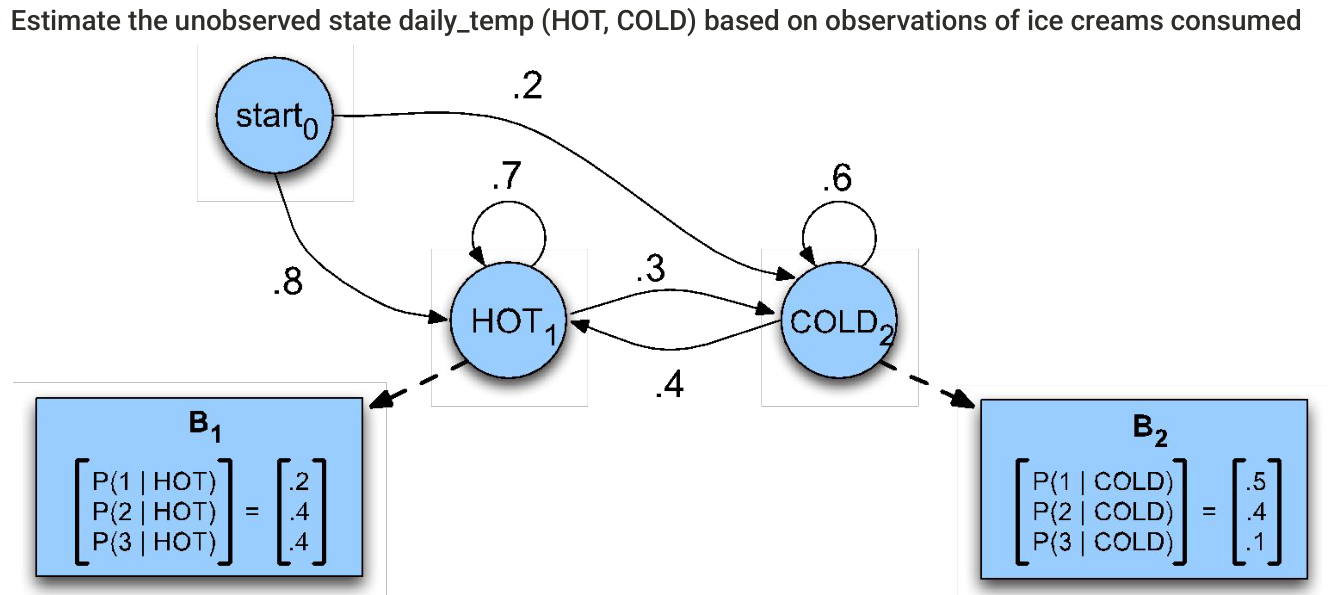
\includegraphics[width=\textwidth,height=0.72\textheight,keepaspectratio]{assets/New-Lecture-STT/cs224s_lec9_slide_19.png}
\end{frame}


\begin{frame}{Audio Feature Extraction: MFCCs}
  \begin{columns}[T]
    \begin{column}{0.51\textwidth}
      \begin{itemize}
        \item Human hearing is not equally sensitive to all frequency bands
        \item Less sensitive at higher frequencies, $>$1000~Hz
        \item I.e.\ human perception of frequency is non-linear
      \end{itemize}
    \end{column}
    \begin{column}{0.48\textwidth}
      \centering
      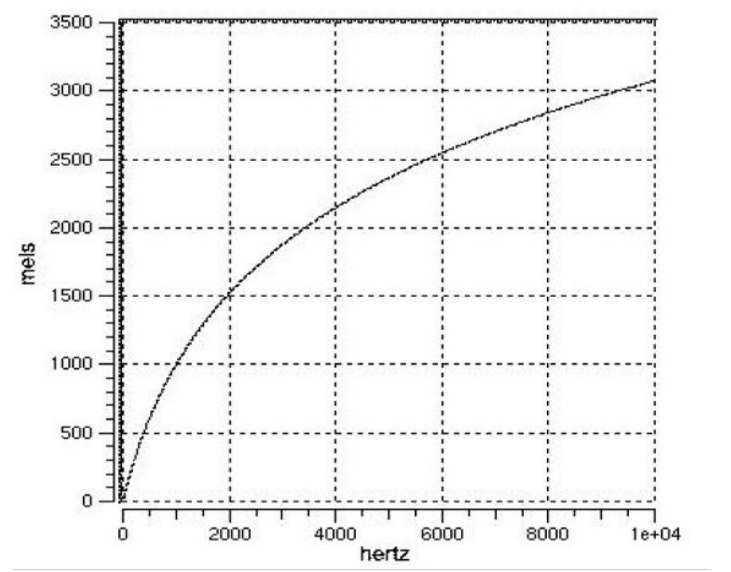
\includegraphics[width=0.95\textwidth]{assets/New-Lecture-STT/cs224s_lec9_slide_22.png}
    \end{column}
  \end{columns}
\end{frame}

% --- Stanford CS224S lec9, slide 23 ---
\begin{frame}{Mel Filter Bank Processing}
  \centering
  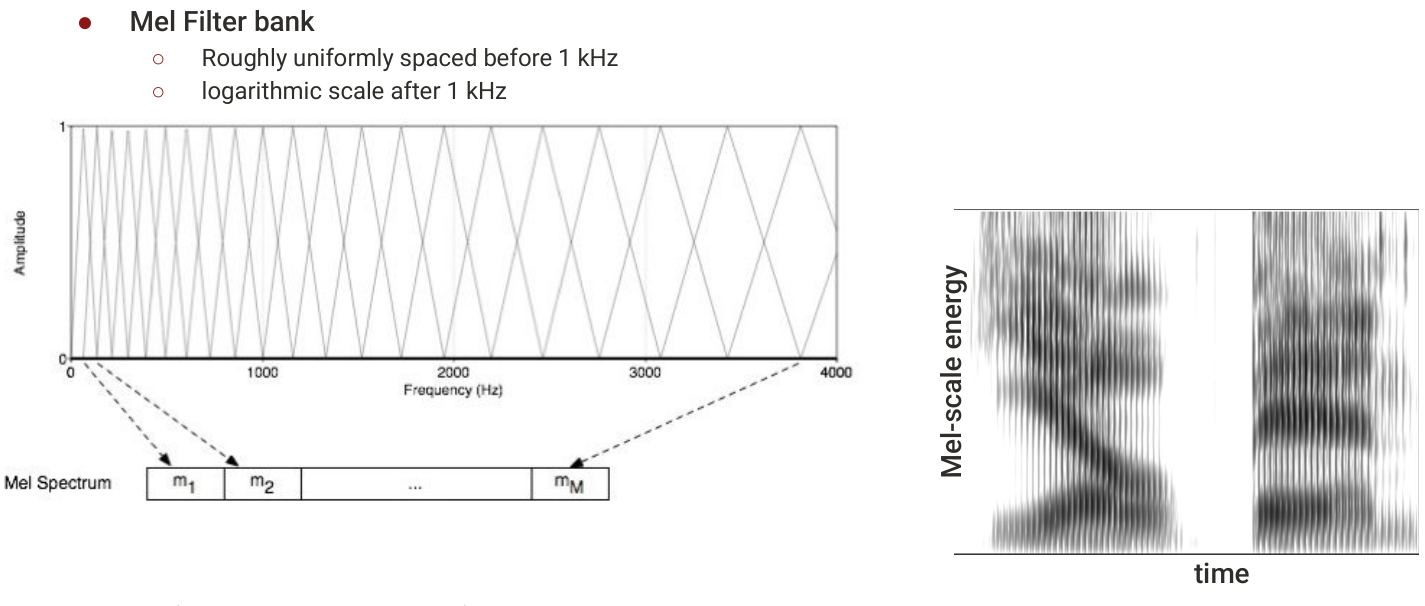
\includegraphics[width=\textwidth,height=0.92\textheight,keepaspectratio]{assets/New-Lecture-STT/cs224s_lec9_slide_23.png}
\end{frame}


% GMM Acoustic Models and Phonetic States
\begin{frame}{Gaussians Mixtures for Acoustic Modeling}
  \centering
  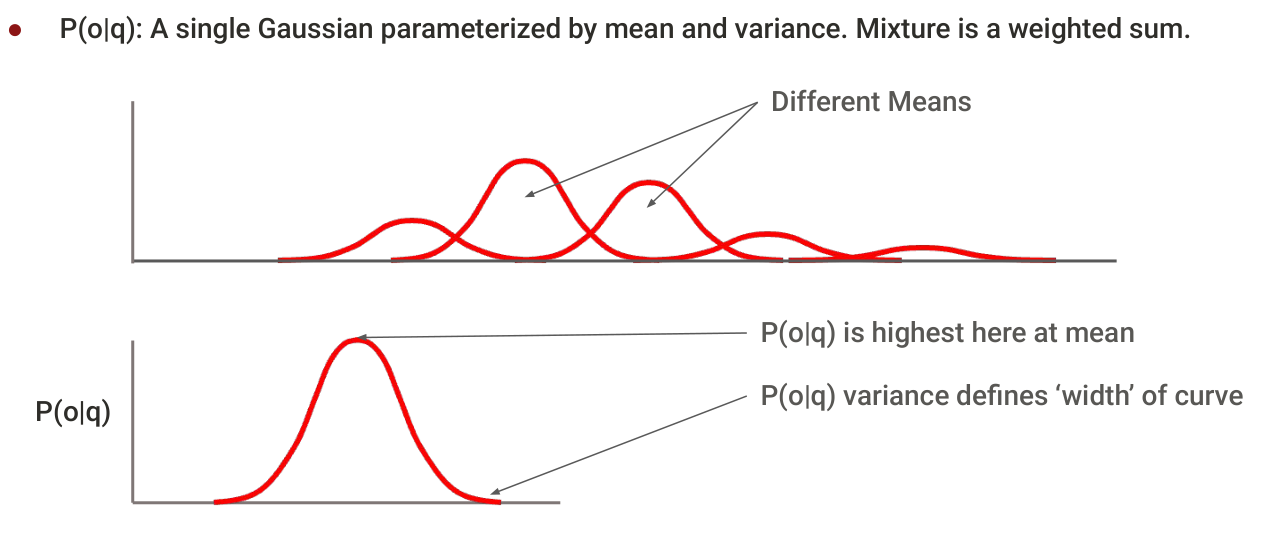
\includegraphics[width=\textwidth,height=0.92\textheight,keepaspectratio]{assets/New-Lecture-STT/cs224s_lec9_slide_27.png}
\end{frame}

% --- Stanford CS224S lec9, slide 28 ---
\begin{frame}{GMMs}
  \centering
  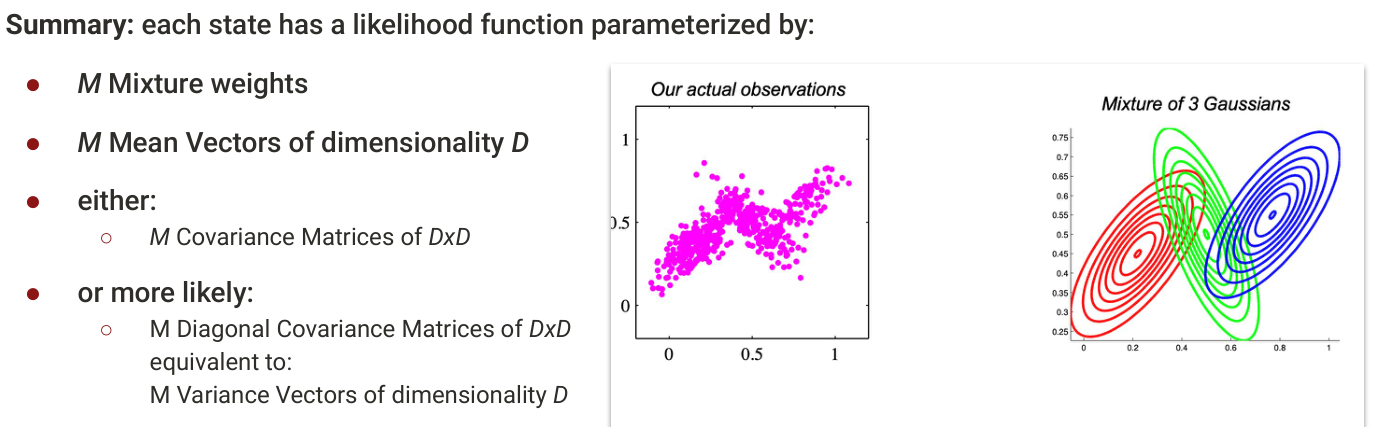
\includegraphics[width=\textwidth,height=0.92\textheight,keepaspectratio]{assets/New-Lecture-STT/cs224s_lec9_slide_28.png}
\end{frame}

% --- Stanford CS224S lec9, slide 40 ---
\begin{frame}{Training an HMM system (Viterbi)}
  \begin{itemize}
    \item \textbf{Given our lexicon + HMM structure, and some acoustic model, we can:}
    \begin{itemize}
      \item Generate the best alignment of HMM states to acoustic observations
    \end{itemize}
    \item \textbf{With an alignment of HMM states to observations:}
    \begin{itemize}
      \item Build a new acoustic model. Treat current state/obs mapping as training data+labels
      \item This acoustic model is hopefully better than previous one
    \end{itemize}
    \item \textbf{Repeat the align $\rightarrow$ rebuild acoustic model process until convergence}
    \begin{itemize}
      \item Add parameters / complexity to acoustic model each iteration
    \end{itemize}
  \end{itemize}
\end{frame}
